% Owner: Hasan  |  Task: T7  |  Drafted by ORCA agents, finalised by the owner.
% Condensed 2026-11-08 (tasks/condense.md); full text at git tag survey-full-v1.
\section{Feature- and Relation-Based Distillation}
\label{sec:feature}

% INTERPRETATION: the suitability judgments and cross-method comparisons in this section are our synthesis; method descriptions and reported values are tied to the cited records.

Feature methods expose intermediate representations and relation methods transfer structure among examples. Methods differ in whether they match feature values directly, transform them, or match invariants such as pairwise distances (Fig.~\ref{fig:knowledge-types}). Direct matching assumes corresponding features; looser constraints can accommodate heterogeneous architectures.

\subsection{Feature alignment and projector design}

FitNets guide a thin student with intermediate ``hints'' through a learned regressor that reconciles dimensions, giving early layers a signal output-only KD lacks; a poorly chosen layer or projection can constrain rather than help \citep{romero2015fitnets}. ReviewKD aggregates multi-stage teacher features into review representations for each student stage, at the cost of extra feature paths \citep{chen2021reviewkd}. SimKD projects the student's penultimate feature into the teacher classifier's space and reuses the teacher classifier on the student's learned feature representation; this does not guarantee the same input-space decision boundary, and the head remains at inference (78.08\%) \citep{chen2022simkd}. The 2024 projector study (SRD) warns that a projector's gain is entangled with normalisation and loss design, so projector-only ablations should come before crediting a loss; it reports 76.44\% with RandAugment (78.37\% with non-standard SSKD teachers, not comparable) \citep{miles2024projector}.
% src: SimKD T1; miles2024projector T5 (g-gap.md row); SRD (IJCV) T8

\subsection{Cross-architecture transfer}

For heterogeneous pairs, the common strategy is to relax direct channel matching: supervision moves to a shared space or to invariants that do not assume stage-wise correspondence. OFA-KD projects intermediate student features into the logit space \citep{hao2023ofakd}. Such methods often lack results on the standard homogeneous pairs.

\subsection{Relational and contrastive transfer}

RKD matches pairwise distances and angles between examples rather than coordinates, freeing channel correspondence at the cost of batch-dependent targets \citep{park2019rkd}. CRD maximises teacher--student agreement for the same example against negatives, which needs negative-sampling memory and is sensitive to the sampling protocol \citep{tian2020crd}. VRM builds affinity graphs over real and virtual samples and prunes unreliable edges, so its gains depend on augmentation quality (78.76\%) \citep{zhang2025vrm}. TopoKD distils feature-space topology through persistence diagrams (75.40\%; 73.60\% on ImageNet, above the 73.31\% teacher it prints) \citep{kim2024topkd}. WKD-F applies a Wasserstein distance to Gaussian feature distributions \citep{lv2024wkd}.
% src: VRM T1; TopKD (ICML 2024) T1/T3

\subsection{Comparison of feature and relation methods}

Methods can be compared by where supervision attaches, what relationship it preserves, and what extra training work it requires. FitNets and ReviewKD use intermediate features; SimKD reuses the teacher classifier; RKD and CRD compare examples, while VRM uses virtual neighbours. Projectors, negative sampling and virtual samples add computation or protocol sensitivity. For same-family compression, FitNets, ReviewKD or SimKD fit when stages or the classifier are compatible. For cross-family pairs, methods that relax channel matching trade it for assumptions about the shared space. RKD, CRD and VRM make the batch or distribution the unit of supervision, so batch size, negatives and virtual samples become error sources. These are heuristics, not a ranking. Standard-pair results are in \S\ref{sec:benchmarks} and supplementary Table~S2.


% Fig. 3: Three targets of distillation; representative methods follow the section taxonomy.
\begin{figure}[t]
\centering
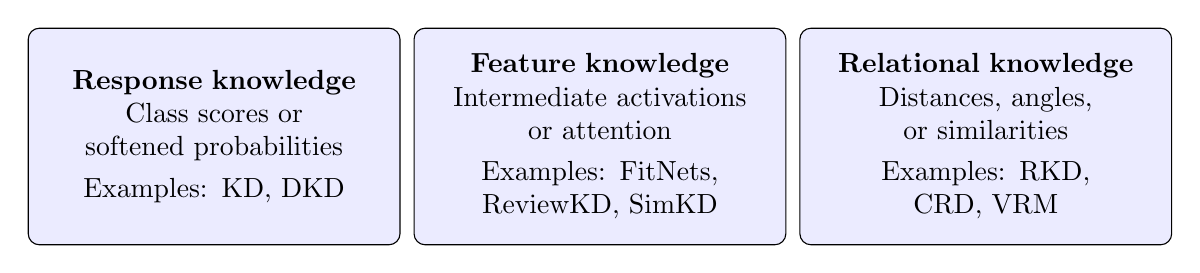
\begin{tikzpicture}[box/.style={draw,rounded corners,align=center,text width=4.3cm,minimum height=2.75cm,inner sep=6pt}]
\node[box,fill=blue!8] (response) at (0,0) {\textbf{Response knowledge}\\Class scores or\\softened probabilities\\[3pt]Examples: KD, DKD};
\node[box,fill=blue!8] (feature) at (4.9,0) {\textbf{Feature knowledge}\\Intermediate activations\\or attention\\[3pt]Examples: \mbox{FitNets}, \mbox{ReviewKD}, \mbox{SimKD}};
\node[box,fill=blue!8] (relation) at (9.8,0) {\textbf{Relational knowledge}\\Distances, angles,\\or similarities\\[3pt]Examples: RKD, CRD, VRM};
\end{tikzpicture}
\caption{Three principal knowledge targets: output responses, internal representations, and structure between examples. A method may combine targets; the categories describe its principal transferred signal.}
\label{fig:knowledge-types}
\end{figure}

